\documentclass[student, noshadow, lsr, aspectratio=169]{ITR_LSR_slides}
%\documentclass[student]{ITRslides}
% use class option 'aspectratio=43' for 4:3 layout

\addbibresource{ref.bib}
\graphicspath{{pics/}{logos/}}

\title{Titel der Präsentation}
\presenter{S. Student}

\supervisor{B. Betreuer}
\typeofpres{Zwischenbericht Masterarbeit}

\usepackage[bigfiles]{media9} %option bigfiles not needed for xelatex, runs without problems on ubuntu14

%%%%%%%%%%%%%%%%%%%%%%%%%%%%%%%%%%%%%%%%%%%%%%%%%%%%%%%%%%%%%%%%%%%%%%%%%%%%%%%%

\begin{document}


\begin{frame}
    \titlepage
\end{frame}


\section{Einführung}

\begin{frame}
	\frametitle{Einführung1}
	\begin{itemize}
 		\item $y=x^2+\sqrt{z}+\int_{a}^{b}{xyz}$
	\end{itemize}
\end{frame}

\begin{frame}
	\frametitle{Einführung2}

%\begin{figure}[htb]
%\centering
%\psfrag{q1}[Bl][Bl]{\small $\alpha$}
%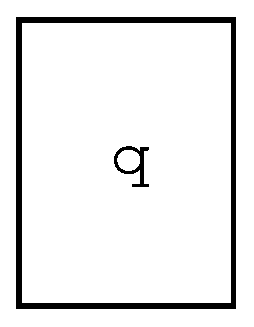
\includegraphics[width=0.9\textwidth]{samplefigure.eps}
%\caption{Sample Figure}
%\end{figure}

\end{frame}

\begin{frame}
	\frametitle{Related Work}
    Normal cite: \cite{8242464}\\
	Bigger cite: \scite{buss11}\\
	Multiple  authors: \cite[3]{bauer09}
\end{frame}

\section{Methoden}

\begin{frame}
	\frametitle{Methoden1}
	\begin{itemize}
		\item a
		\item b
	\end{itemize}
\end{frame}

\begin{frame}
	\frametitle{Methoden2}
	\begin{itemize}
		\item a
	\end{itemize}
\end{frame}

\begin{frame}
	\frametitle{Methoden3}
	\begin{itemize}
		\item a
	\end{itemize}
\end{frame}

\section{Ergebnisse}

\begin{frame}
	\frametitle{Ergebnisse1}
	...
\end{frame}

\begin{frame}
	\frametitle{Ergebnisse2}
	...
\end{frame}

% VIDEO: both examples below show a figure where the video will be displayed. 
% This figure could be a still picture of the video, giving a hint on what the video will show. 
% Usage of such a figure can be useful in case the presentation is likely to be printed as e.g. a handout 

% NOTE: the folder containing the videos MUST BE INSIDE the presentation folder, otherwise the videos might not show up in the presentation.
% Also: the videos cannot be displayed on ubuntu, use e.g. the windows imperator to check whether the videos work

%video example1
{
    \usebackgroundtemplate{\includemedia[width=12.8cm,height=9.6cm,activate=onclick,]{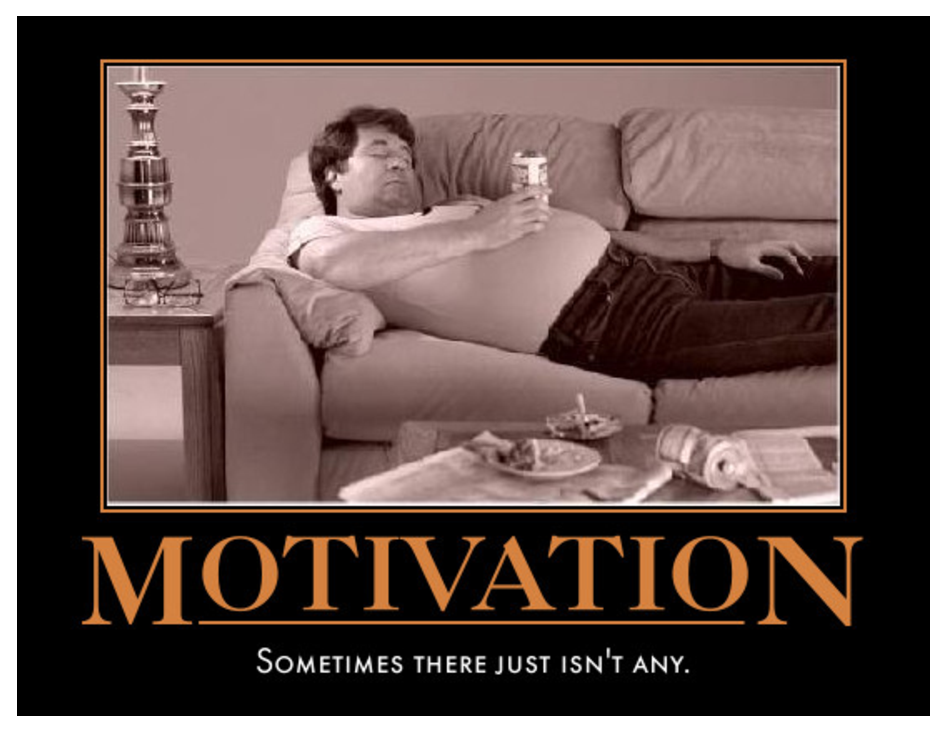
\includegraphics{motivation}}{movie/example_video_short.swf}} 
    \begin{frame}[plain]
    \end{frame}
}

%video example2
% \begin{frame}
% 	\frametitle{Example video}
% \includemedia[height=.5\textwidth]{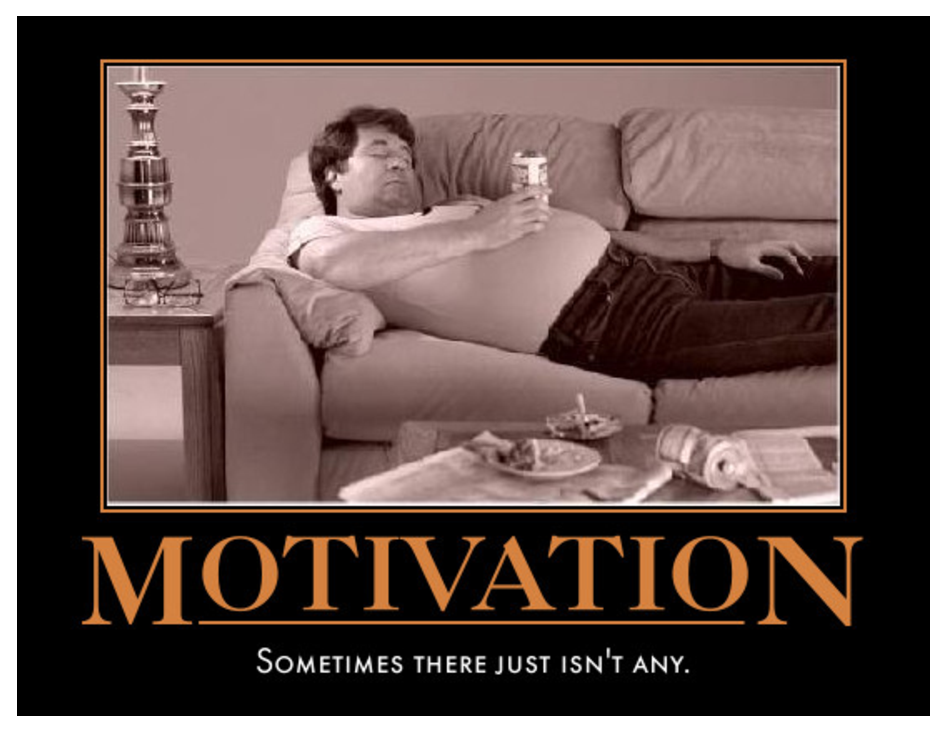
\includegraphics[height=.5\textwidth]{motivation.eps}}{movie/example_video_short.swf} 
% \end{frame}

\section{Zusammenfassung}

\begin{frame}
	\frametitle{Zusammenfassung}
	...
\end{frame}
\appendix
%\nocite{buss11}
%\nocite{bauer09}
\begin{frame}
	\frametitle{Referenzen}
	%\tiny
	%\bibliographystyle{plain}
	%\bibliography{ref}
	\printbibliography
\end{frame}


\end{document}
